\section{Fabrics}
\label{sec:fabrics}

Textile fabrics are the cornerstone of numerous industries, from fashion to aerospace, shaping products that touch every aspect of daily life. With over 25,000 distinct fabric types, each defined by unique textures, strengths, and appearances, their accurate identification is essential for quality assurance and innovation \citep{Kampouris2016}. In our research on fabric classification using deep learning, we depend on a thorough understanding of fabrics, their diverse categories, and how they differ from the fibres that constitute them. This section lays the groundwork for our work, which employs advanced \ac{CNN} and \ac{ViT} models to automate fabric identification with high precision, as detailed in Section~\ref{sec:motivation}.

\subsection{Definition of Fabrics}
\label{subsec:fabric_definition}

Fabrics are the finished materials of textile production, crafted by weaving, knitting, or felting fibres into cohesive sheets. They serve as the foundation for countless applications—clothing, upholstery, medical textiles, and even high-performance materials like parachute canopies. Fabrics are engineered to meet specific demands, such as the softness of cotton bedsheets or the resilience of polyester car seats. Their significance spans multiple sectors:
\begin{itemize}
    \item \textbf{Fashion}: Designers select fabrics like silk for elegance or denim for durability.
    \item \textbf{Home Furnishings}: Wool and synthetic blends are used in curtains, carpets, and sofas for comfort and longevity.
    \item \textbf{Automotive}: Nylon and polyester fabrics ensure safety and durability in seat covers and airbags.
    \item \textbf{Medical}: Cotton and non-woven synthetics are critical for surgical gowns and bandages, prioritizing hygiene.
    \item \textbf{Aerospace and Defense}: High-strength fabrics like Kevlar provide lightweight, durable solutions \citep{Nayak2020}.
\end{itemize}

The sheer variety of fabrics, with over 25,000 types, underscores the challenge of manual identification \citep{Kampouris2016}. Our research addresses this by leveraging datasets like the Fabrics Dataset (3,692 images across 24 classes) and the Fabrics OCT Dataset (1,476 images of cotton, wool, and polyester) to train models that distinguish fabrics with up to 98.34\% accuracy, as discussed in Section~\ref{sec:results} \citep{Jatav2025}.

\subsection{Types of Fabrics}
\label{subsec:fabric_types}

Fabrics are categorized based on their construction, source, or intended use, resulting in a vast array of types with distinct properties. We classify them into several key groups:
\begin{itemize}
    \item \textbf{Natural Fabrics}: Sourced from plants or animals, these include:
        \begin{itemize}
            \item \textbf{Cotton}: Soft and breathable, ideal for t-shirts and linens.
            \item \textbf{Wool}: Warm and resilient, used in sweaters and blankets.
            \item \textbf{Silk}: Lustrous and smooth, favored in luxury fashion.
            \item \textbf{Linen}: Crisp and lightweight, suitable for summer apparel.
        \end{itemize}
    \item \textbf{Synthetic Fabrics}: Chemically produced, these include:
        \begin{itemize}
            \item \textbf{Polyester}: Durable and wrinkle-resistant, common in sportswear and upholstery.
            \item \textbf{Nylon}: Strong and elastic, used in stockings and ropes.
            \item \textbf{Acrylic}: Wool-like, a cost-effective option for knitwear.
        \end{itemize}
    \item \textbf{Blended Fabrics}: Combinations like cotton-polyester, balancing comfort and durability.
    \item \textbf{Specialty Fabrics}: Designed for specific purposes, such as Kevlar for bulletproof vests or Gore-Tex for waterproof clothing.
\end{itemize}

Each fabric type exhibits unique visual and structural characteristics, which our deep learning models exploit for classification. For example, the fine weave of silk contrasts with denim’s coarse texture, enabling our dual-branch \ac{CNN}-\ac{ViT} model to achieve high performance on datasets like TextileNet (760,949 images across 18 fabric classes) \citep{Zhong2023, Jatav2025}.

\subsection{Fibres: The Building Blocks}
\label{subsec:fibres}

Fibres are the raw materials that form fabrics, consisting of thread-like or filament structures capable of being spun into yarns. They are the individual threads in a tapestry, each contributing to the final material’s properties. Fibres are classified as:
\begin{itemize}
    \item \textbf{Natural Fibres}:
        \begin{itemize}
            \item \textbf{Cotton}: Plant-derived, soft and absorbent.
            \item \textbf{Wool}: Sheep-sourced, known for insulation and elasticity.
            \item \textbf{Silk}: Silkworm-produced, fine and lustrous.
            \item \textbf{Jute}: Plant-based, coarse and strong, used in sacks.
        \end{itemize}
    \item \textbf{Synthetic Fibres}:
        \begin{itemize}
            \item \textbf{Polyester}: Chemically synthesized, resistant to wrinkles.
            \item \textbf{Nylon}: Durable and elastic, ideal for heavy-duty uses.
            \item \textbf{Acrylic}: Wool-mimicking, used in affordable knitwear.
        \end{itemize}
\end{itemize}

Fibres are spun into yarns, which are woven, knitted, or felted to create fabrics. This process resembles constructing a house: fibres are the bricks, yarns the walls, and fabrics the completed structure \citep{Jatav2025}. The microscopic properties of fibres, visible in datasets like the Fabrics OCT Dataset, influence how fabrics appear in images used for our classification models \citep{Sabuncu2022}.

\subsection{Differences Between Fibres and Fabrics}
\label{subsec:differences}

Fibres and fabrics, though interconnected, are fundamentally distinct. Fibres are the single, thread-like units serving as raw materials, while fabrics are the finished, two-dimensional sheets created from them. Key differences include:
\begin{itemize}
    \item \textbf{Composition}: Fibres are individual strands (e.g., a cotton fibre). Fabrics combine multiple fibres, often blending types (e.g., cotton-polyester fabric).
    \item \textbf{Structure}: Fibres are one-dimensional threads; fabrics are two-dimensional with complex patterns like weaves or knits.
    \item \textbf{Applications}: Fibres form yarns, which create fabrics. Fabrics are directly used in products like clothing or upholstery.
    \item \textbf{Properties}: Fibre properties (e.g., cotton’s absorbency) shape the fabric, but the fabric’s final characteristics depend on construction. A tightly woven cotton fabric differs from a loosely knitted one.
\end{itemize}

This distinction is pivotal for our research, as our models analyze fabric-level images, capturing weave patterns rather than fibre structures. For instance, our models distinguish silk’s smooth weave from wool’s fuzzy texture in the Fabrics Dataset, achieving high accuracy by focusing on fabric features \citep{Kampouris2016, Jatav2025}. Figure~\ref{fig:fabric_construction} illustrates this process, showing how fibres are transformed into fabrics.

% \begin{figure}[H]
%     \centering
%     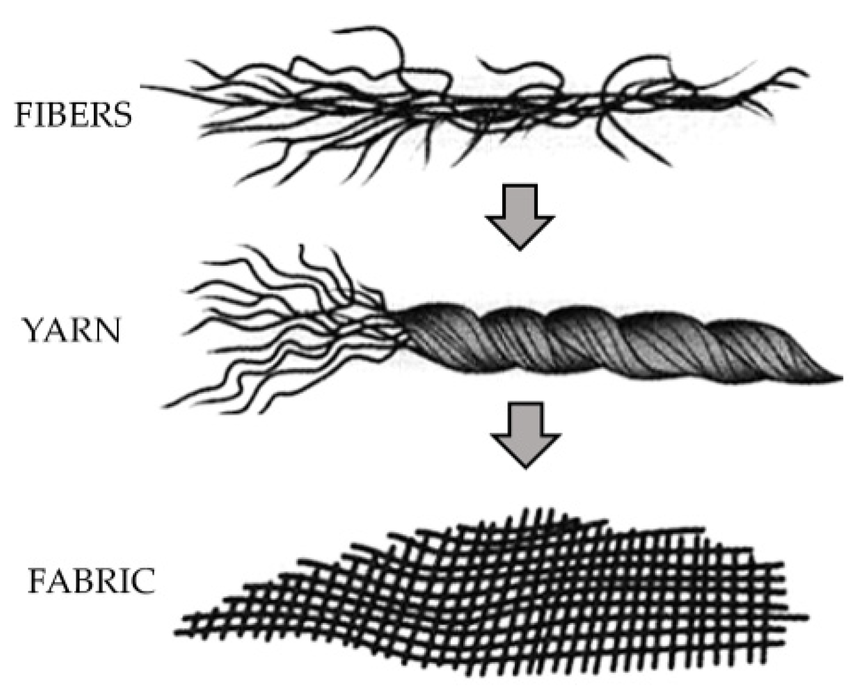
\includegraphics[width=0.6\textwidth]{fabric_construction}
%     \caption{Construction of Fabric from Fibres \citep{Jatav2025}}
%     \label{fig:fabric_construction}
% \end{figure}

\subsection{Relevance to Fabric Classification}
\label{subsec:relevance}

A deep understanding of fabrics and fibres is essential for our automated classification efforts. The diversity of fabric types, each with unique visual signatures, makes manual identification labor-intensive, particularly in industries demanding rapid quality checks. Our research tackles this challenge by training models like VGG16, MobileNetV2, and a custom \ac{CNN}-\ac{ViT} architecture on diverse datasets, achieving up to 98.34\% accuracy \citep{Jatav2025}. By accurately identifying fabrics like cotton, wool, and polyester, we contribute to streamlining processes in textiles, from e-commerce to manufacturing, as explored further in Section~\ref{sec:results}.